\section{类SampledSpectrum}\label{sec:类SampledSpectrum}
\refvar{SampledSpectrum}{}用\refvar{CoefficientSpectrum}{}基础结构
来表示在起始和结束波长之间均匀间隔采样的SPD。
波长覆盖范围从400nm到700nm——人类视觉系统最为敏感的可见光谱范围。
样本数量60一般足够为渲染准确表示复杂的SPD
(见“扩展阅读”一节了解SPD采样率要求的背景)。
因此,第一个样本表示波长范围$[400,405)$,第二个表示$[405,410)$,以此类推。
这些值很容易在此处按需修改。
\begin{lstlisting}
`\initcode{Spectrum Utility Declarations}{=}\initnext{SpectrumUtilityDeclarations}`
static const int `\initvar{sampledLambdaStart}{}` = 400;
static const int `\initvar{sampledLambdaEnd}{}` = 700;
static const int `\initvar{nSpectralSamples}{}` = 60;
\end{lstlisting}
\begin{lstlisting}
`\refcode{Spectrum Declarations}{+=}\lastnext{SpectrumDeclarations}`
class `\initvar{SampledSpectrum}{}` : public `\refvar{CoefficientSpectrum}{}`<`\refvar{nSpectralSamples}{}`> {
public:
    `\refcode{SampledSpectrum Public Methods}{}`
private:
    `\refcode{SampledSpectrum Private Data}{}`
};
\end{lstlisting}

通过从类\refvar{CoefficientSpectrum}{}继承,
\refvar{SampledSpectrum}{}自动拥有之前定义的所有基本光谱算术运算符。
留待为它定义的主要方法是从光谱数据初始化它以及将它表示的SPD转换为其他光谱表示(例如RGB)。
用常数SPD初始化它的构造函数很简单。
\begin{lstlisting}
`\initcode{SampledSpectrum Public Methods}{=}\initnext{SampledSpectrumPublicMethods}`
`\refvar{SampledSpectrum}{}`(`\refvar{Float}{}` v = 0.f) : `\refvar{CoefficientSpectrum}{}`(v) { }
\end{lstlisting}

光谱数据经常以一组样本$(\lambda_i,v_i)$提供给我们,
其中第$i$个样本有在波长$\lambda_i$处的某值$v_i$。
一般而言,样本可能有不规则间隔,可能比\refvar{SampledSpectrum}{}要存储的更多或更少
(见pbrt发行中路径{\ttfamily scenes/spds}下\sidenote{译者注:笔者没有找到该路径。}
pbrt所用的各种SPD,它们许多都有不规则间隔)。

方法\refvar{FromSampled}{()}取用在
给定波长{\ttfamily lambda}处的SPD样本值{\ttfamily v}数组
并用它们定义分段线性函数来表示SPD。
对于\refvar{SampledSpectrum}{}的每个SPD样本,
它用下面定义的功能函数\refvar{AverageSpectrumSamples}{()}
来计算分段线性函数在每个SPD样本对应的波长范围上的均值。
\begin{lstlisting}
`\refcode{SampledSpectrum Public Methods}{+=}\lastnext{SampledSpectrumPublicMethods}`
static `\refvar{SampledSpectrum}{}` `\initvar{FromSampled}{}`(const `\refvar{Float}{}` *lambda,
                                   const `\refvar{Float}{}` *v, int n) {
    `\refcode{Sort samples if unordered, use sorted for returned spectrum}{}`
    `\refvar{SampledSpectrum}{}` r;
    for (int i = 0; i < `\refvar{nSpectralSamples}{}`; ++i) {
        `\refcode{Compute average value of given SPD over th sample's range}{}`
    }
    return r;
}
\end{lstlisting}

函数\refvar{AverageSpectrumSamples}{()}要求值$(\lambda_i,v_i)$按波长排序。
{\initvar{SpectrumSamplesSorted}{()}}函数检查它们是不是;
如果不是,则{\initvar{SortSpectrumSamples}{()}}对它们排序。
注意我们为排序的样本分配新存储而不改变调用者传入的值;
一般而言,对于该函数(不需要担心其特定实现的这些要求)的用户
这样做可能并不是期望的行为。
我们这里不会介绍这两个函数的实现,因为它们很简单。
\begin{lstlisting}
`\initcode{Sort samples if unordered, use sorted for returned spectrum}{=}`
if (!`\refvar{SpectrumSamplesSorted}{}`(lambda, v, n)) {
    std::vector<`\refvar{Float}{}`> slambda(&lambda[0], &lambda[n]);
    std::vector<`\refvar{Float}{}`> sv(&v[0], &v[n]);
    `\refvar{SortSpectrumSamples}{}`(&slambda[0], &sv[0], n);
    return `\refvar{FromSampled}{}`(&slambda[0], &sv[0], n);
}
\end{lstlisting}

为计算第$i$个光谱样本的值,我们计算其对应的波长范围——
{\ttfamily lambda0}到{\ttfamily lambda1}——
并用函数\refvar{AverageSpectrumSamples}{()}计算该范围给定分段线性SPD的均值。
这是采样和重构的1D实例,第\refchap{采样与重构}会讨论该话题的更多细节。
\begin{lstlisting}
`\initcode{Compute average value of given SPD over th sample's range}{=}`
`\refvar{Float}{}` lambda0 = `\refvar{Lerp}{}`(`\refvar{Float}{}`(i) / `\refvar{Float}{}`(`\refvar{nSpectralSamples}{}`), 
                     `\refvar{sampledLambdaStart}{}`, `\refvar{sampledLambdaEnd}{}`);
`\refvar{Float}{}` lambda1 = `\refvar{Lerp}{}`(`\refvar{Float}{}`(i + 1) / `\refvar{Float}{}`(`\refvar{nSpectralSamples}{}`), 
                     `\refvar{sampledLambdaStart}{}`, `\refvar{sampledLambdaEnd}{}`);
r.`\refvar[CoefficientSpectrum::c]{c}{}`[i] = `\refvar{AverageSpectrumSamples}{}`(lambda, v, n, lambda0, lambda1);
\end{lstlisting}

\reffig{5.2}展示了\refvar{AverageSpectrumSamples}{()}采用的基础方法:
它在部分或完全位于波长范围内的样本间的每个线性段上迭代,
从{\ttfamily lambdaStart}到{\ttfamily lambdaEnd}。
对于每个这样的分段,它计算其范围上的均值,
用该段覆盖的波长范围缩放该均值,最后求这些值的和。
最终均值是该和除以整个波长范围。
\begin{figure}[htbp]
    \centering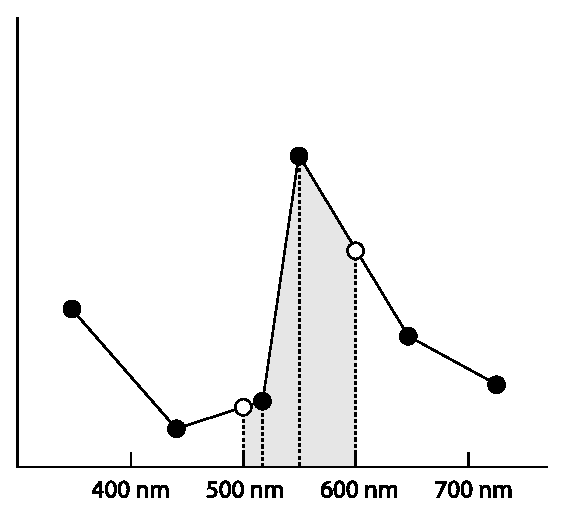
\includegraphics[width=0.4\linewidth]{chap05/IrregularSPDresample.eps}
    \caption{当重采样不规则定义的SPD时,我们需要计算由SPD样本定义的
        分段线性函数的均值。这里,我们想求从500nm到600nm的均值——图像下的阴影区。
        函数\refvar{AverageSpectrumSamples}{()}通过计算该图中虚线表示的每个区域的面积来完成。}
    \label{fig:5.2}
\end{figure}

\begin{lstlisting}
`\initcode{Spectrum Method Definitions}{=}\initnext{SpectrumMethodDefinitions}`
`\refvar{Float}{}` `\initvar{AverageSpectrumSamples}{}`(const `\refvar{Float}{}` *lambda, const `\refvar{Float}{}` *vals,
        int n, `\refvar{Float}{}` lambdaStart, `\refvar{Float}{}` lambdaEnd) {
    `\refcode{Handle cases with out-of-bounds range or single sample only}{}`
    `\refvar{Float}{}` sum = 0;
    `\refcode{Add contributions of constant segments before/after samples}{}`
    `\refcode{Advance to first relevant wavelength segment}{}`
    `\refcode{Loop over wavelength sample segments and add contributions}{}`
    return sum / (lambdaEnd - lambdaStart);
}
\end{lstlisting}

该函数从检查和处理极端情况开始,即求均值的波长范围
超出了提供的波长范围或只有单个样本进而均值计算是平凡的情况。
我们假设SPD在超出提供的采样范围外有常值(在两个端点的值);
如果这对于特定数据集不是一个合理的假设,则提供的数据应该在端点处有显式值(例如)0。
\begin{lstlisting}
`\initcode{Handle cases with out-of-bounds range or single sample only}{=}`
if (lambdaEnd   <= lambda[0])     return vals[0];
if (lambdaStart >= lambda[n - 1]) return vals[n - 1];
if (n == 1) return vals[0];
\end{lstlisting}

处理了这些情况后,下一步是检查看求均值的范围是否有部分超出第一个和/或最后一个样本值。
如果是,则我们累积常数段的贡献,用超出边界的波长范围缩放它。
\begin{lstlisting}
`\initcode{Add contributions of constant segments before/after samples}{=}`
if (lambdaStart < lambda[0])
    sum += vals[0] * (lambda[0] - lambdaStart);
if (lambdaEnd > lambda[n-1])
    sum += vals[n - 1] * (lambdaEnd - lambda[n - 1]);
\end{lstlisting}

现在我们推进到首个索引{\ttfamily i},
插值范围的起始波长重合于从$\lambda_i$到$\lambda_{i+1}$的一段。
这里更高效的实现是用二叉搜索而不是线性搜索
\footnote{甚至更高效的实现是利用一个事实即调用代码一般会需要
    在一段相邻波长范围上插值后的值,并可能在单次调用中接收了全部范围。
    然后可以为下一次插值从上一结尾处开始逐步寻找起始索引。}。
然而,该代码目前只在场景初始化时调用,所以目前不优化它不会影响渲染性能。
\begin{lstlisting}
`\initcode{Advance to first relevant wavelength segment}{=}`
int i = 0;
while (lambdaStart > lambda[i + 1]) ++i;
\end{lstlisting}

下面的循环在与求均值的范围重合的每个线性段上迭代。
对于每一段,它都通过求函数在这两点上取值的均值来
计算在波长范围{\ttfamily segLambdaStart}到{\ttfamily segLambdaEnd}上的均值。
该值依次用{\ttfamily interp()}计算,它是在给定波长的两个端点间线性插值的匿名函数。

下面的{\ttfamily std::min()}和{\ttfamily std::max()}调用计算波长范围以在该段内做平均;
注意它们自然地处理了{\ttfamily lambdaStart}、{\ttfamily lambdaEnd}或两者都在当前段内的情况。
\begin{lstlisting}
`\initcode{Loop over wavelength sample segments and add contributions}{=}`
auto interp = [lambda, vals](`\refvar{Float}{}` w, int i) {
    return `\refvar{Lerp}{}`((w - lambda[i]) / (lambda[i + 1] - lambda[i]),
                vals[i], vals[i + 1]);
};
for (; i+1 < n && lambdaEnd >= lambda[i]; ++i) {
    `\refvar{Float}{}` segLambdaStart = std::max(lambdaStart, lambda[i]);
    `\refvar{Float}{}` segLambdaEnd =   std::min(lambdaEnd,   lambda[i + 1]);
    sum += 0.5 * (interp(segLambdaStart, i) + interp(segLambdaEnd, i)) *
        (segLambdaEnd - segLambdaStart);
}
\end{lstlisting}

\subsection{XYZ颜色}\label{sub:XYZ颜色}
人类视觉系统的一个非凡性质是可只用三个浮点数为人类感知表示颜色。
颜色感知的\keyindex{三色刺激理论}{tristimulus theory}{}说
用三个值$x_{\lambda},y_{\lambda}$和$z_{\lambda}$就能为人类观察者准确表示所有可见SPD。
给定发射SPD即$S(\lambda)$,通过积分它们与\keyindex{光谱匹配曲线}{spectral matching curve}{}
$X(\lambda),Y(\lambda)$和$Z(\lambda)$的积可算得这些值:
\begin{align}\label{eq:5.1}
    x_{\lambda} & =\int\limits_{\lambda}{S(\lambda)X(\lambda)\mathrm{d}\lambda}\, ,\nonumber \\
    y_{\lambda} & =\int\limits_{\lambda}{S(\lambda)Y(\lambda)\mathrm{d}\lambda}\, ,          \\
    z_{\lambda} & =\int\limits_{\lambda}{S(\lambda)Z(\lambda)\mathrm{d}\lambda}\, .\nonumber
\end{align}

这些曲线是由国际照明委员会\sidenote{译者注:法文Commission Internationale de l'Éclairage,
    英文International Commission on Illumination,是有关光学、照明、颜色和色度空间科学领域的国际组织,成立于1913年。}(CIE)
规范化机构在一系列以人类为测试对象的实验后决定的并画于\reffig{5.3}中。
一般认为这些匹配曲线通常类似于人类视网膜中三种色敏视锥细胞\sidenote{译者注:原文 color-sensitive cone。}的响应。
惊人的是,有截然不同分布的SPD可能有非常接近的$x_{\lambda},y_{\lambda}$和$z_{\lambda}$值。
对于人类观察者,这样的SPD实际上有一样的视觉呈现。
这样的光谱对称为\keyindex{条件等色}{metamer}{}。
\begin{figure}[htbp]
    \centering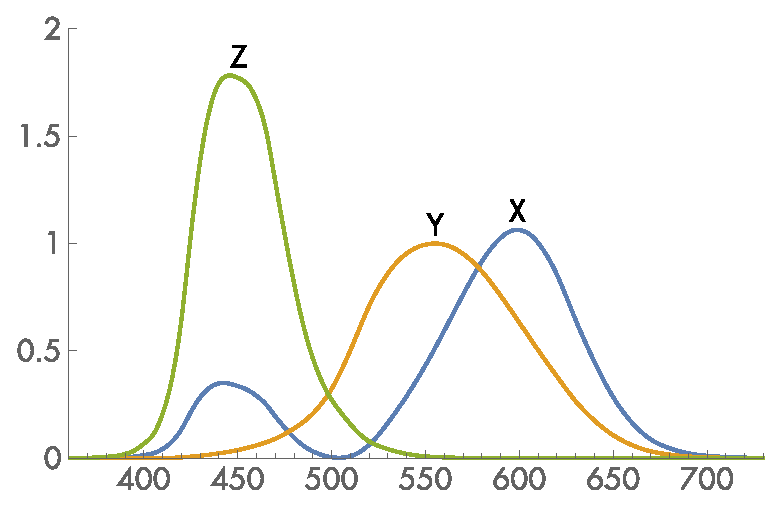
\includegraphics[width=0.5\linewidth]{chap05/matching-xyz.eps}
    \caption{对任意SPD计算XYZ值。用\refeq{5.1}让SPD与三个匹配曲线的每一个
    相乘并在其非零范围上积分以计算$x_{\lambda},y_{\lambda}$和$z_{\lambda}$值。}
    \label{fig:5.3}
\end{figure}

这给我们带来了关于光谱功率分布表示的一个微妙之处。
大部分颜色空间都希望模型颜色是对人类可见的,进而根据颜色感知的三色刺激理论只需用三个系数。
尽管XYZ能很好地表示要对人类观察者显示的给定SPD,
但它对于光谱计算而言{\itshape 不是}特别好的基函数集。
例如,尽管XYZ值能很好地分别描述柠檬皮或荧光灯的感知颜色(回想\reffig{5.1}),
但它们各自的XYZ值之积给出的XYZ颜色可能明显不同于用其SPD更精确的表示相乘再计算出的XYZ值。

